%%%%%%%%%%%%%%%%%%%%%%%%%%%%%%%%%%%%%%%%%%%%%%%
%
% Template per Elaborato di Laurea
% DISI - Dipartimento di Ingegneria e Scienza dell’Informazione
%
% update 2015-09-10
%
% Per la generazione corretta del 
% pdflatex nome_file.tex
% bibtex nome_file.aux
% pdflatex nome_file.tex
% pdflatex nome_file.tex
%
%%%%%%%%%%%%%%%%%%%%%%%%%%%%%%%%%%%%%%%%%%%%%%%

% formato FRONTE RETRO
\documentclass[epsfig,a4paper,11pt,titlepage,twoside,openany]{book}
\usepackage{epsfig}
\usepackage{plain}
\usepackage{setspace}
\usepackage[paperheight=29.7cm,paperwidth=21cm,outer=1.5cm,inner=2.5cm,top=2cm,bottom=2cm]{geometry} % per definizione layout
\usepackage{titlesec} % per formato custom dei titoli dei capitoli
\usepackage[hidelinks]{hyperref}

%%%%%%%%%%%%%%
% supporto lettere accentate
%
%\usepackage[latin1]{inputenc} % per Windows;
\usepackage[utf8x]{inputenc} % per Linux (richiede il pacchetto unicode);
%\usepackage[applemac]{inputenc} % per Mac.

\singlespacing

\usepackage[italian]{babel}

\begin{document}

  % nessuna numerazione
  \pagenumbering{gobble} 
  \pagestyle{plain}

\thispagestyle{empty}

\begin{center}
  \begin{figure}[h!]
    \centerline{
\psfig{file=logo_unitn.png,width=0.6\textwidth}}
  \end{figure}

  \vspace{2 cm} 

  \LARGE{Department of Information Engineering and Computer Science\\}

  \vspace{1 cm} 
  \Large{Master’s Degree in Computer Science
    %Ingegneria dell'Informazione e delle Comunicazioni
    %Ingegneria dell'Informazione e Organizzazione d'Impresa
    %Ingegneria Elettronica e delle Telecomunicazioni
  }

  \vspace{2 cm} 
  \Large\textsc{Final Dissertation\\} 
  \vspace{1 cm} 
  \hrule
  \vspace{0.5 cm} 
  \Huge{A novel cloud based prototype for diagnostic electrocardiography EHR-ready with webservices interoperability\\}
  \vspace{0.5 cm} 
  \hrule
  %\Large{\it{Sottotitolo (alcune volte lungo - opzionale)}}


  \vspace{2 cm} 
  \begin{tabular*}{\textwidth}{ c @{\extracolsep{\fill}} c }
  \Large{Supervisor} & \Large{Student}\\
  \Large{Giandomenico Nollo}& \Large{Samuele Malavasi}\\
  \Large{Enrico Blanzieri}
  \end{tabular*}

  \vspace{2 cm} 

  \Large{Academic year 2016/2017}
  
\end{center}



  \clearpage
 
%%%%%%%%%%%%%%%%%%%%%%%%%%%%%%%%%%%%%%%%%%%%%%%%%%%%%%%%%%%%%%%%%%%%%%%%%%
%%%%%%%%%%%%%%%%%%%%%%%%%%%%%%%%%%%%%%%%%%%%%%%%%%%%%%%%%%%%%%%%%%%%%%%%%%
%% Nota
%%%%%%%%%%%%%%%%%%%%%%%%%%%%%%%%%%%%%%%%%%%%%%%%%%%%%%%%%%%%%%%%%%%%%%%%%%
%% Sezione Ringraziamenti opzionale
%%%%%%%%%%%%%%%%%%%%%%%%%%%%%%%%%%%%%%%%%%%%%%%%%%%%%%%%%%%%%%%%%%%%%%%%%%
%%%%%%%%%%%%%%%%%%%%%%%%%%%%%%%%%%%%%%%%%%%%%%%%%%%%%%%%%%%%%%%%%%%%%%%%%%
  \thispagestyle{empty}

  \begin{center}
    {\bf \Huge Ringraziamenti}
  \end{center}

  \vspace{4cm}

  \emph{
    ...thanks to...
  }
  \clearpage
  \pagestyle{plain} % nessuna intestazione e pie pagina con numero al centro

%%%%%%%%%%%%%%%%%%%%%%%%%%%%%%%%%%%%%%%%%%%%%%%%%%%%%%%%%%%%%%%%%%%%%%%%%%
%%%%%%%%%%%%%%%%%%%%%%%%%%%%%%%%%%%%%%%%%%%%%%%%%%%%%%%%%%%%%%%%%%%%%%%%%%
%% Nota
%%%%%%%%%%%%%%%%%%%%%%%%%%%%%%%%%%%%%%%%%%%%%%%%%%%%%%%%%%%%%%%%%%%%%%%%%%
%% Sezione Citazioni opzionale
%%%%%%%%%%%%%%%%%%%%%%%%%%%%%%%%%%%%%%%%%%%%%%%%%%%%%%%%%%%%%%%%%%%%%%%%%%
%%%%%%%%%%%%%%%%%%%%%%%%%%%%%%%%%%%%%%%%%%%%%%%%%%%%%%%%%%%%%%%%%%%%%%%%%%
  \thispagestyle{empty}
%\topskip0pt
\vspace*{\fill}
\emph{
    You're progressing on something and that's what it's all about. You wanna keep moving, having a progress in your life.
}
\hfill Ueli Steck
\vspace*{\fill}



  \clearpage
  \pagestyle{plain} % nessuna intestazione e pie pagina con numero al centro

  
  % inizio numerazione pagine in numeri arabi
  \mainmatter

%%%%%%%%%%%%%%%%%%%%%%%%%%%%%%%%%%%%%%%%%%%%%%%%%%%%%%%%%%%%%%%%%%%%%%%%%%
%%%%%%%%%%%%%%%%%%%%%%%%%%%%%%%%%%%%%%%%%%%%%%%%%%%%%%%%%%%%%%%%%%%%%%%%%%
%% Nota
%%%%%%%%%%%%%%%%%%%%%%%%%%%%%%%%%%%%%%%%%%%%%%%%%%%%%%%%%%%%%%%%%%%%%%%%%%
%% Si ricorda che il numero massimo di facciate e' 30.
%% Nel conteggio delle facciate sono incluse 
%%   indice
%%   abstract
%%   capitoli
%% Dal conteggio delle facciate sono escluse
%%   frontespizio
%%   ringraziamenti
%%   allegati    
%%%%%%%%%%%%%%%%%%%%%%%%%%%%%%%%%%%%%%%%%%%%%%%%%%%%%%%%%%%%%%%%%%%%%%%%%%
%%%%%%%%%%%%%%%%%%%%%%%%%%%%%%%%%%%%%%%%%%%%%%%%%%%%%%%%%%%%%%%%%%%%%%%%%%

    % indice
    \tableofcontents
    \clearpage
    
    
          
    % gruppo per definizone di successione capitoli senza interruzione di pagina
    \begingroup
      % nessuna interruzione di pagina tra capitoli
      % ridefinizione dei comandi di clear page
      %\renewcommand{\cleardoublepage}{} 
      %\renewcommand{\clearpage}{} 
      % redefinizione del formato del titolo del capitolo
      % da formato
      %   Capitolo X
      %   Titolo capitolo
      % a formato
      %   X   Titolo capitolo
      
      \titleformat{\chapter}
      {\normalfont\Huge\bfseries}{\thechapter}{1em}{}
        
      \titlespacing*{\chapter}{0pt}{0.59in}{0.02in}
      \titlespacing*{\section}{0pt}{0.20in}{0.02in}
      \titlespacing*{\subsection}{0pt}{0.10in}{0.02in}
      
      % abstract
      \thispagestyle{empty}
\begin{center}
    {\chapter*{Abstract}} % senza numerazione
\end{center}
\label{abstract}

\addcontentsline{toc}{chapter}{Abstract} % da aggiungere comunque all'indice
The idea of this thesis was born during my internship in Cardioline Spa, a developer and producer Heart Activity technological products company based in Trento.\\Cloud-based technologies and software interoperability are powerful and interesting tools in order to improve the IT offer and keep up with the times for companies. The Italian Digital Agenda included a strict plan for the public health digitalization which implies the development of a Clinical Document Repository. Actually the italian version has just seen a first release, in December 2017.\\Cardioline is already selling a software support to its customers, enabling different kinds of electrocardiography exams: the company provides hospitals, clinics and various stakeholders with a set of Hearth Activity Monitoring machines and an ad hoc WebApplication on their LAN. The current approach is limited by the private Network boundaries, the server availability and resources, in favor of an high control, security level and compatibility with legacy applications.\\The goal is to reengineer the softwares, from one-tier to multi-tier, from a stand-alone to a cloud-based infrastructure keeping the same security level and taking into account the laws regulating sensitive data.\\ The challenge starts by making a realistic proposal solution for Cardioline by exploring the current market offer. Later it will be to develop the proposed solution by respecting each of the constraints.\\ \\My work in particular was focused on managing EHR (Electronic Health Record) documents, formats, standards, files and communication interfaces to the Italian Clinical Document Repository (FSE - Fascicolo Sanitario Elettronico).\\Furthermore, I dealt with REST-Services (REpresentational State Transfer) in order to manage the new infrastructure, involving third-parties software on the client side.\\A prototype solution has been built to show the possible immediate innovation that can be achieved, suitable for any other company managing Electronic Health Data, which requires to be always available, from any place, with immediate application, and easy to handle in an increasingly smart way.\\ \\
The thesis is divided in three main parts. The first one gives the reader on overview of the current state of the art for the technologies being used. A section is dedicated to cloud computing and how is it available to customers and developers. Section 1.2 explains how different systems communicate each other via different web service implementation. The end of the first part, section 1.3, describes briefly what is an electrocardiogram and how is the exam performed until its digitalization and storage into approved national repositories. The second part, is more focused on the specific problem faced, in the first part the analysis and system requirement are illustrated while in the last part there's a detailed explanation of the developed prototype.\\The third part concludes this work by outlining the carried innovation and ideas for further improvements.
      \clearpage
%%%%%%%%%%%%%%%%%%%%%%%%%%%%%%%%%%%%%%%%%%%%%%%%%%%%%%%%%%%%%%%%%%%%%%%%%%
%%%%%%%%%%%%%%%%%%%%%%%%%%%%%%%%%%%%%%%%%%%%%%%%%%%%%%%%%%%%%%%%%%%%%%%%%%
%% Nota
%%%%%%%%%%%%%%%%%%%%%%%%%%%%%%%%%%%%%%%%%%%%%%%%%%%%%%%%%%%%%%%%%%%%%%%%%%
%% Abstract e' un breve riassunto del lavoro svolto dove si descrive 
%% l’obiettivo, l’oggetto della tesi, le metodologie e 
%% le tecniche usate, i dati elaborati e la spiegazione delle conclusioni 
%% alle quali siete arrivati.
%% Il abstract dell’elaborato consiste al massimo di 3 pagine e deve contenere le seguenti informazioni: 
%%   contesto e motivazioni
%%   breve riassunto del problema affrontato
%%   tecniche utilizzate e/o sviluppate
%%   risultati raggiunti, sottolineando il contributo personale del laureando/a
%%%%%%%%%%%%%%%%%%%%%%%%%%%%%%%%%%%%%%%%%%%%%%%%%%%%%%%%%%%%%%%%%%%%%%%%%%
%%%%%%%%%%%%%%%%%%%%%%%%%%%%%%%%%%%%%%%%%%%%%%%%%%%%%%%%%%%%%%%%%%%%%%%%%%      
      
      %%%%%%%%%%%%%%%%%%%%%%%%%%%%%%%%
      % lista dei capitoli
      %
      % \input oppure \include
      %
      
      %% -1	\part{part}
%% 0	\chapter{chapter}
%% 1	\section{section}
%% 2	\subsection{subsection}
%% 3	\subsubsection{subsubsection}
%% 4	\paragraph{paragraph}
%% 5	\subparagraph{subparagraph}
%% \part and \chapter are only available in report and book document classes

\bibliography{biblio}
    \bibliographystyle{plain}

\chapter{Introduction}
ciccio~\label{cha:manna}
reference~\ref{cha:manna}

\section{State Of The Art}
\subsection{Ecg Solutions}
\subsubsection{Clinically-used 12-lead ECG}
12-Lead Ecg is on of the most used methodology in clinical cardiac medicine, it consists on attaching 10 electrodes on the surface of the limbs and the chest and therefore generates 12-lead: 12 groups of signals.\\
Traditionally each instrument generates vendor-specific waveform data formats which are compressed or encrypted by their algorithms.
\subsubsection{ECG Digitalization}
In 1989-1990 European, American and Japanese manufacturers jointly worked and agreed \cite{Chronaki}
\subsection{Cloud Computing Application To Medical Device}


\section{Thesis Structure}
\label{sec:greetings}

Hello!
I greeted in section~\ref{sec:greetings}.
      %% 2. 
%% (a)  (b) Implementation
%% (c) Workflow
%% (d) Long-term preservation

\chapter{Electronic health record}
\label{cha:intro}

Lorem ipsum dolor sit amet, consectetur adipiscing elit. Donec sed nunc orci. Aliquam nec nisl vitae sapien pulvinar dictum quis non urna. Suspendisse at dui a erat aliquam vestibulum. Quisque ultrices pellentesque pellentesque. Pellentesque egestas quam sed blandit tempus. Sed congue nec risus posuere euismod. Maecenas ut lacus id mauris sagittis egestas a eu dui. Class aptent taciti sociosqu ad litora torquent per conubia nostra, per inceptos himenaeos. Pellentesque at ultrices tellus. Ut eu purus eget sem iaculis ultricies sed non lorem. Curabitur gravida dui eget ex vestibulum venenatis. Phasellus gravida tellus velit, non eleifend justo lobortis eget. 
\cite{coulouris}

Donec eu ipsum id lorem consectetur luctus ac a nisi. Curabitur volutpat, metus id porta ultrices, felis lacus consectetur justo, ut gravida arcu ex in purus. Pellentesque vitae sapien ac nisl porttitor pellentesque eu sed elit. Sed maximus lectus eu eros ultricies accumsan. Quisque congue, nisi in dictum cursus, ante nisl molestie eros, in ultrices eros tellus sit amet augue. Interdum et malesuada fames ac ante ipsum primis in faucibus. Nam finibus leo sit amet purus vehicula, eget facilisis turpis convallis. Vivamus varius tincidunt turpis, id venenatis arcu maximus ut. Aenean euismod eros ac nibh facilisis, nec imperdiet ex suscipit.
\cite{dalal}


\section{Accredited organization}
\section{Implementation}
\section{Workflow}
\section{Long-term preservation}

\label{sec:context}

Lorem ipsum dolor sit amet, consectetur adipiscing elit. Donec sed nunc orci. Aliquam nec nisl vitae sapien pulvinar dictum quis non urna. Suspendisse at dui a erat aliquam vestibulum. Quisque ultrices pellentesque pellentesque. Pellentesque egestas quam sed blandit tempus. Sed congue nec risus posuere euismod. Maecenas ut lacus id mauris sagittis egestas a eu dui. Class aptent taciti sociosqu ad litora torquent per conubia nostra, per inceptos himenaeos. Pellentesque at ultrices tellus. Ut eu purus eget sem iaculis ultricies sed non lorem. Curabitur gravida dui eget ex vestibulum venenatis. Phasellus gravida tellus velit, non eleifend justo lobortis eget.
\cite{ictbusiness}

      \chapter{Cloud Computing}
\section{Definition}
Cloud Computing bas become a buzzword since it is used most of the time improperly and due to the great number of definitions. By the way, cloud computing is not a completely new concept, it is correlated to the 13 years old grid computing paradigm and to distributed systems in general.\cite{foster}\\
A little consensus has been reached defining cloud computing as\\
\textit{A large-scale distributed computing paradigm that is driven by economies of scale, in which a pool of abstracted, virtualized, dynamically-scalable, managed computing power, storage, platforms, and services are delivered on demand to external customers over the Internet.}\\
Concluding, this paradigm with respect to the traditional ones, it is
\begin{itemize}
    \item It is massively scalable
    \item Delivers different levels of services to customers outside the cloud
    \item It is dynamically scaled and configured
\end{itemize}
\cite{foster}
\section{History}

\section{Infrastructure models}
\subsection{Paas}
\subsection{Iaas}
\subsection{Saas}
\subsection{Serverless}
\subsection{Private Cloud}
\subsection{Public Cloud}
\subsection{Hybrid Cloud}
\section{Security}

ciccio~\label{cha:manna}
reference~\ref{cha:manna}

Lorem ipsum dolor sit amet, consectetur adipiscing elit. Donec sed nunc orci. Aliquam nec nisl vitae sapien pulvinar dictum quis non urna. Suspendisse at dui a erat aliquam vestibulum. Quisque ultrices pellentesque pellentesque. Pellentesque egestas quam sed blandit tempus. Sed congue nec risus posuere euismod. Maecenas ut lacus id mauris sagittis egestas a eu dui. Class aptent taciti sociosqu ad litora torquent per conubia nostra, per inceptos himenaeos. Pellentesque at ultrices tellus. Ut eu purus eget sem iaculis ultricies sed non lorem. Curabitur gravida dui eget ex vestibulum venenatis. Phasellus gravida tellus velit, non eleifend justo lobortis eget. 


I greeted in section~\ref{sec:greetings}.
      \chapter{Web Services}
\section{Definition}
\section{Web Services architectures}
\section{EHR Web Services Implementation}


      \chapter{Cardioline Specific ecosystem}
\label{chapter:cardioline_specific_ecosystem}
Cardioline is present on the market from the early 60s, they started developing and producing innovative machines to record the heart acivity. Nowadays their thecnology improved, making their products producing documents in a digital format.
Thus the company started to sell a system able to produce heart rate monitoring digital documents for different methodologies, to forward them to a Software for the storage, to alert the physicians and to let them write their own examination.
\section{Software and Frameworks involved}
The managment software tool is based on .NET platform, since the 32-bit libraries for the SCP-ECG format are microsoft technologies based.
Cardioline provides each customer with a Windows Server Machine running their web applications realized with ASP .NET.
\section{Project target And System requirements}
The scope is to provide future customers with additional features of the managment application, avoiding the burden to keep up and running their own machines and infrastructure while Respecting the European jurisprudence in privacy subject and integrating their system with the national e-healthcare system.
Centralizing such services involved some problems:
\begin{itemize}
    \item High network and computing load
    \item New security policies for data
    \item Adoption of the international HL7 standard
    \item Continuity with legacy software
\end{itemize}
\section{Provider choice}
It has been decided to face the computing and network load problem using Computing Cloud technologies, since they let the developer choose the control degree and customization over the system and how to structure the network.
In particular Cloud Computing providers offers this kinds of services:
\begin{itemize}
    \item Saas
    \item Paas
    \item Iaas
\end{itemize}
\paragraph{Amazon Elestic Beanstalk}
\label{paragraph:amazon_elastic_beanstalk}
[TO DO]
And different kind of network topology such as:
\begin{itemize}
    \item Private cloud
    \item Public cloud
\end{itemize}

%\section{System Architecture}
      \chapter{Implemented Solution}

\section{Amazon Web Services}

\subsection{Architecture}
\begin{figure}[h]
    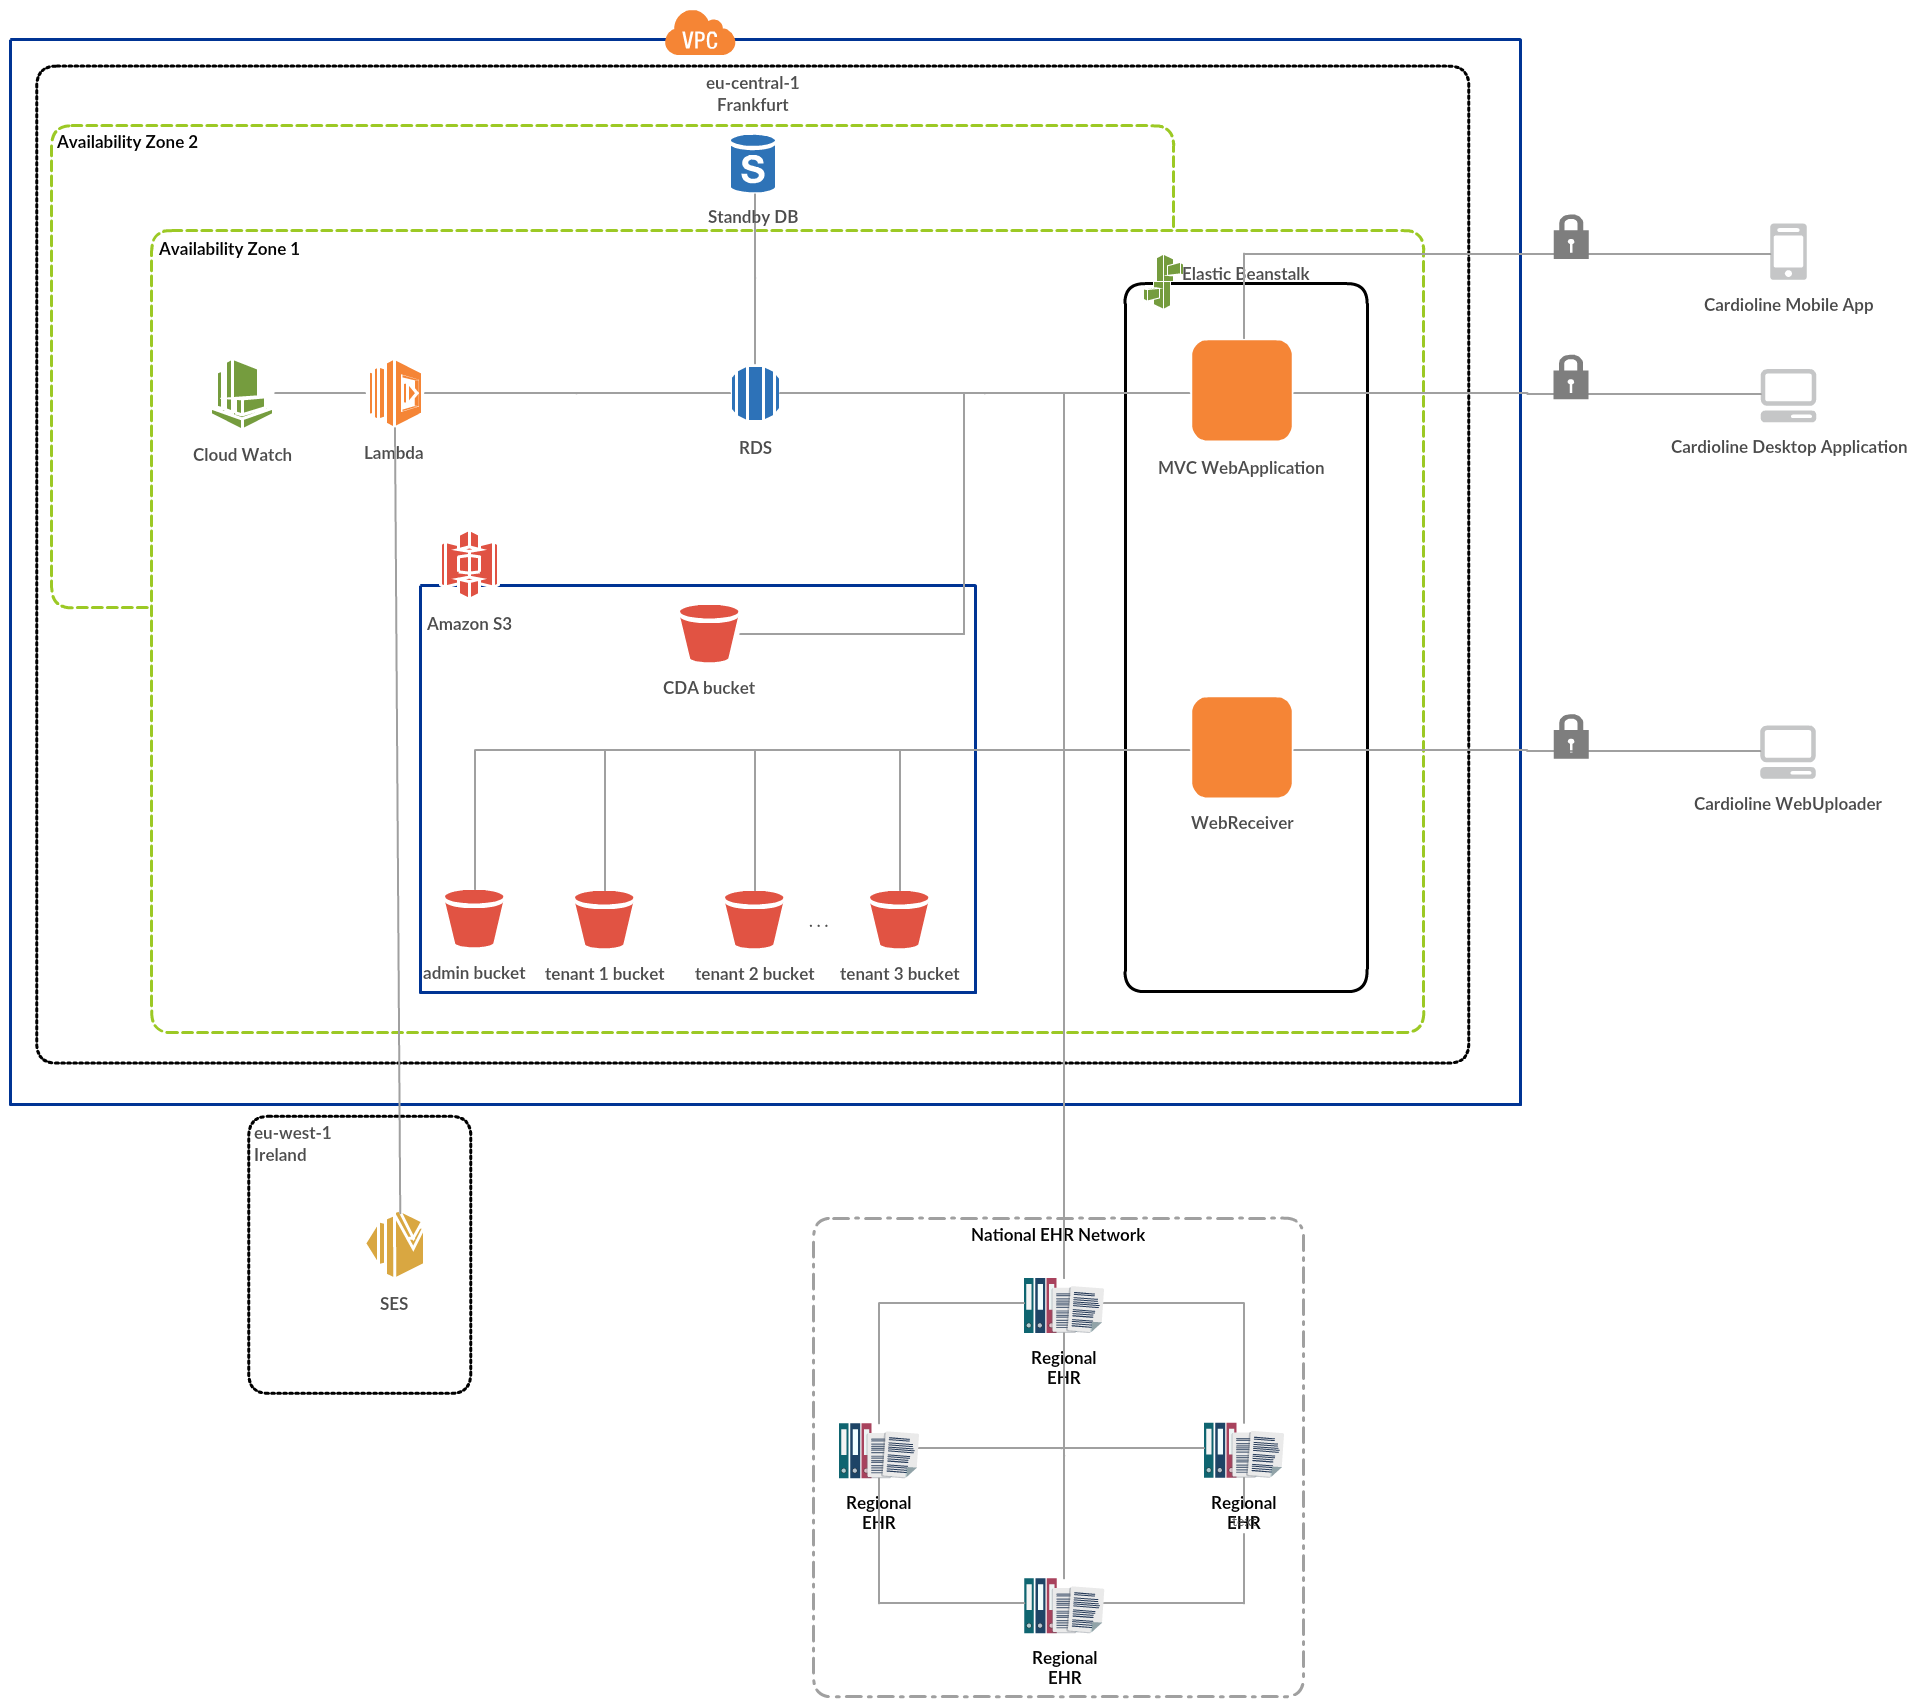
\includegraphics[width=\textwidth]{img/architecture}
    \caption{Architecture Scheme}
    \label{fig:architecture}
\end{figure}
Since Amazon Elastic Beanstalk (EB) has been used as the core component of the system, it has been possible to use an Infrastructure as a Service (IaaS \ref{paragraph:Iaas}) grade of customization, with an easier configuration and building phase as if the system was Platform as a Service (PaaS \ref{paragraph:Paas}) instead.\\
As shown in picture \ref{fig:architecture}, everything but the Amazon Simple Email Service (SES \cite{AmazonSes}) service is hosted in the eu-central-1 region in Frankfurt to reduce latency, minimize costs and keep healthcare data in an European law venue, as in production would be.
The region is divided into availability zones connected each other with low-latency links, to handle potential instance failures by replacing them with the standby ones located in a different availability zone.\\
EB handles the WebServer instances: one for the EcgWebApp, more details in section \ref{paragraph:ecgwebapp} and the other one for Ecg WebReceiver,section \ref{paragraph:ecgwebreceiver}. The interaction is then allowed to authenticated users bounded to their capabilities and role.\\
The persistency is achieved by a Relational Database Service (RDS) running Amazon Aurora DB, a compatible MySql Database organized with a master write replica and several read replicas.
Furthermore, RDS provides a standby and synchronous Database, hosted in another availability zone, that is ready to become the new master in case of failure of the current master.\\
All the assets and static files are read and written from/to AWS S3 relative bucket.\\
The notification system is triggered by DB events and carried on by AWS Lambda functions using Amazon Simple Email Service (SES) as delivery service to final users. This service is not available in the Frankfurt region, hence the Ireland region was chosen.

\section{Ecg Workflow}
\label{section:ecgworkflow}
Resting Electrocardiogram (\ref{paragraph:Resting}) are uploaded from different device types such as mobile phones, desktop computers and Cardioline specific machines to EcgWebApp through a specific REST interface (details about REpresentational State Transter\ref{paragraph:REST}). The exam is stored in a \textit{pending} state and every associated physician notified for the anamnesis provisioning.
The user interface for a physician with anamnesis providing rights logged in is displayed in fig.\ref{fig:todo_anamnesi}.
Once the history of a \textit{pending} exam has been supplied (screenshot at fig.\ref{fig:aggiunta_anamnesi}) it passes to a \textit{ready} state. At this point every associated doctor with review role and permission, usually a cardiologist, is notified and allowed to write its own conclusion, as showed in figure \ref{fig:aggiunta_anamnesi}, and eventually ask for a second opinion from another expert. The exam state is finally set to \textit{confirmed} and the patient doctor notified.
\begin{figure}[h]
    \centering
    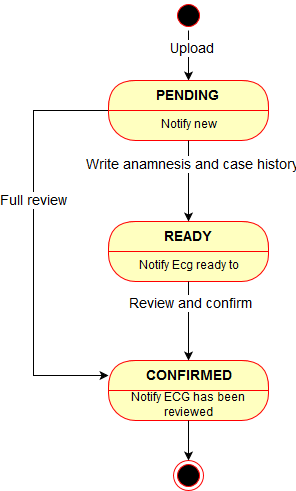
\includegraphics[width=6cm]{img/ECGstatechart}
    \caption{Electrocardiogram State Chart}
    \label{fig:ECGstatechart}
\end{figure}
\clearpage

\section{Interoperability of digital electrocardiograms data}
\paragraph{Resting}
\label{paragraph:Resting}
\paragraph{Cardiac stress test}
\label{paragraph:Cardiac stress test}
\paragraph{Holter}
\label{paragraph:Holter}

\section{Interoperability related architecture components}
The biggest contribution has been provided to the architecture components which interact with an external service. As it is possible to observe in figure \ref{fig:architecture} they are mainly two, EcgWebApp (\ref{paragraph:ecgwebapp}) for resting and cardiac stress test and Ecg WebReceiver (\ref{paragraph:ecgwebreceiver}) for Holter methodology.

\subsection{Web service and application}
These components instances are directly handled by Amazon Web Service Elastic Beanstalk (details at \ref{fig:architecture}): their load balancers and resources are dinamically allocated over the current request, load and configured parameters.\\
They both run on a 64-bit Windows Server 2012 R2 (with 32-bit compatibility) virtual machine executing IIS 8.5.
\paragraph{EcgWebApp}
\label{paragraph:ecgwebapp}
It's a 3-tier deployment architecture (\ref{fig:tiers_diagram}) based on Microsoft ASP .NET MVC framework. Its main components are:
\begin{itemize}
    \item \textit{WebBased UI and REST} - client interface
    \item \textit{WebServer} - handles http requests dispatching and routing to AppServer modules (IIS)
    \item \textit{Application Server} - ASP .NET Framework based business logic
    \item \textit{RDBMS (Relational Database Management System)} - Amazon Aurora and Amazon Simple Cloud Storage Service (S3)
\end{itemize}
\begin{figure}[h]
    \centering
    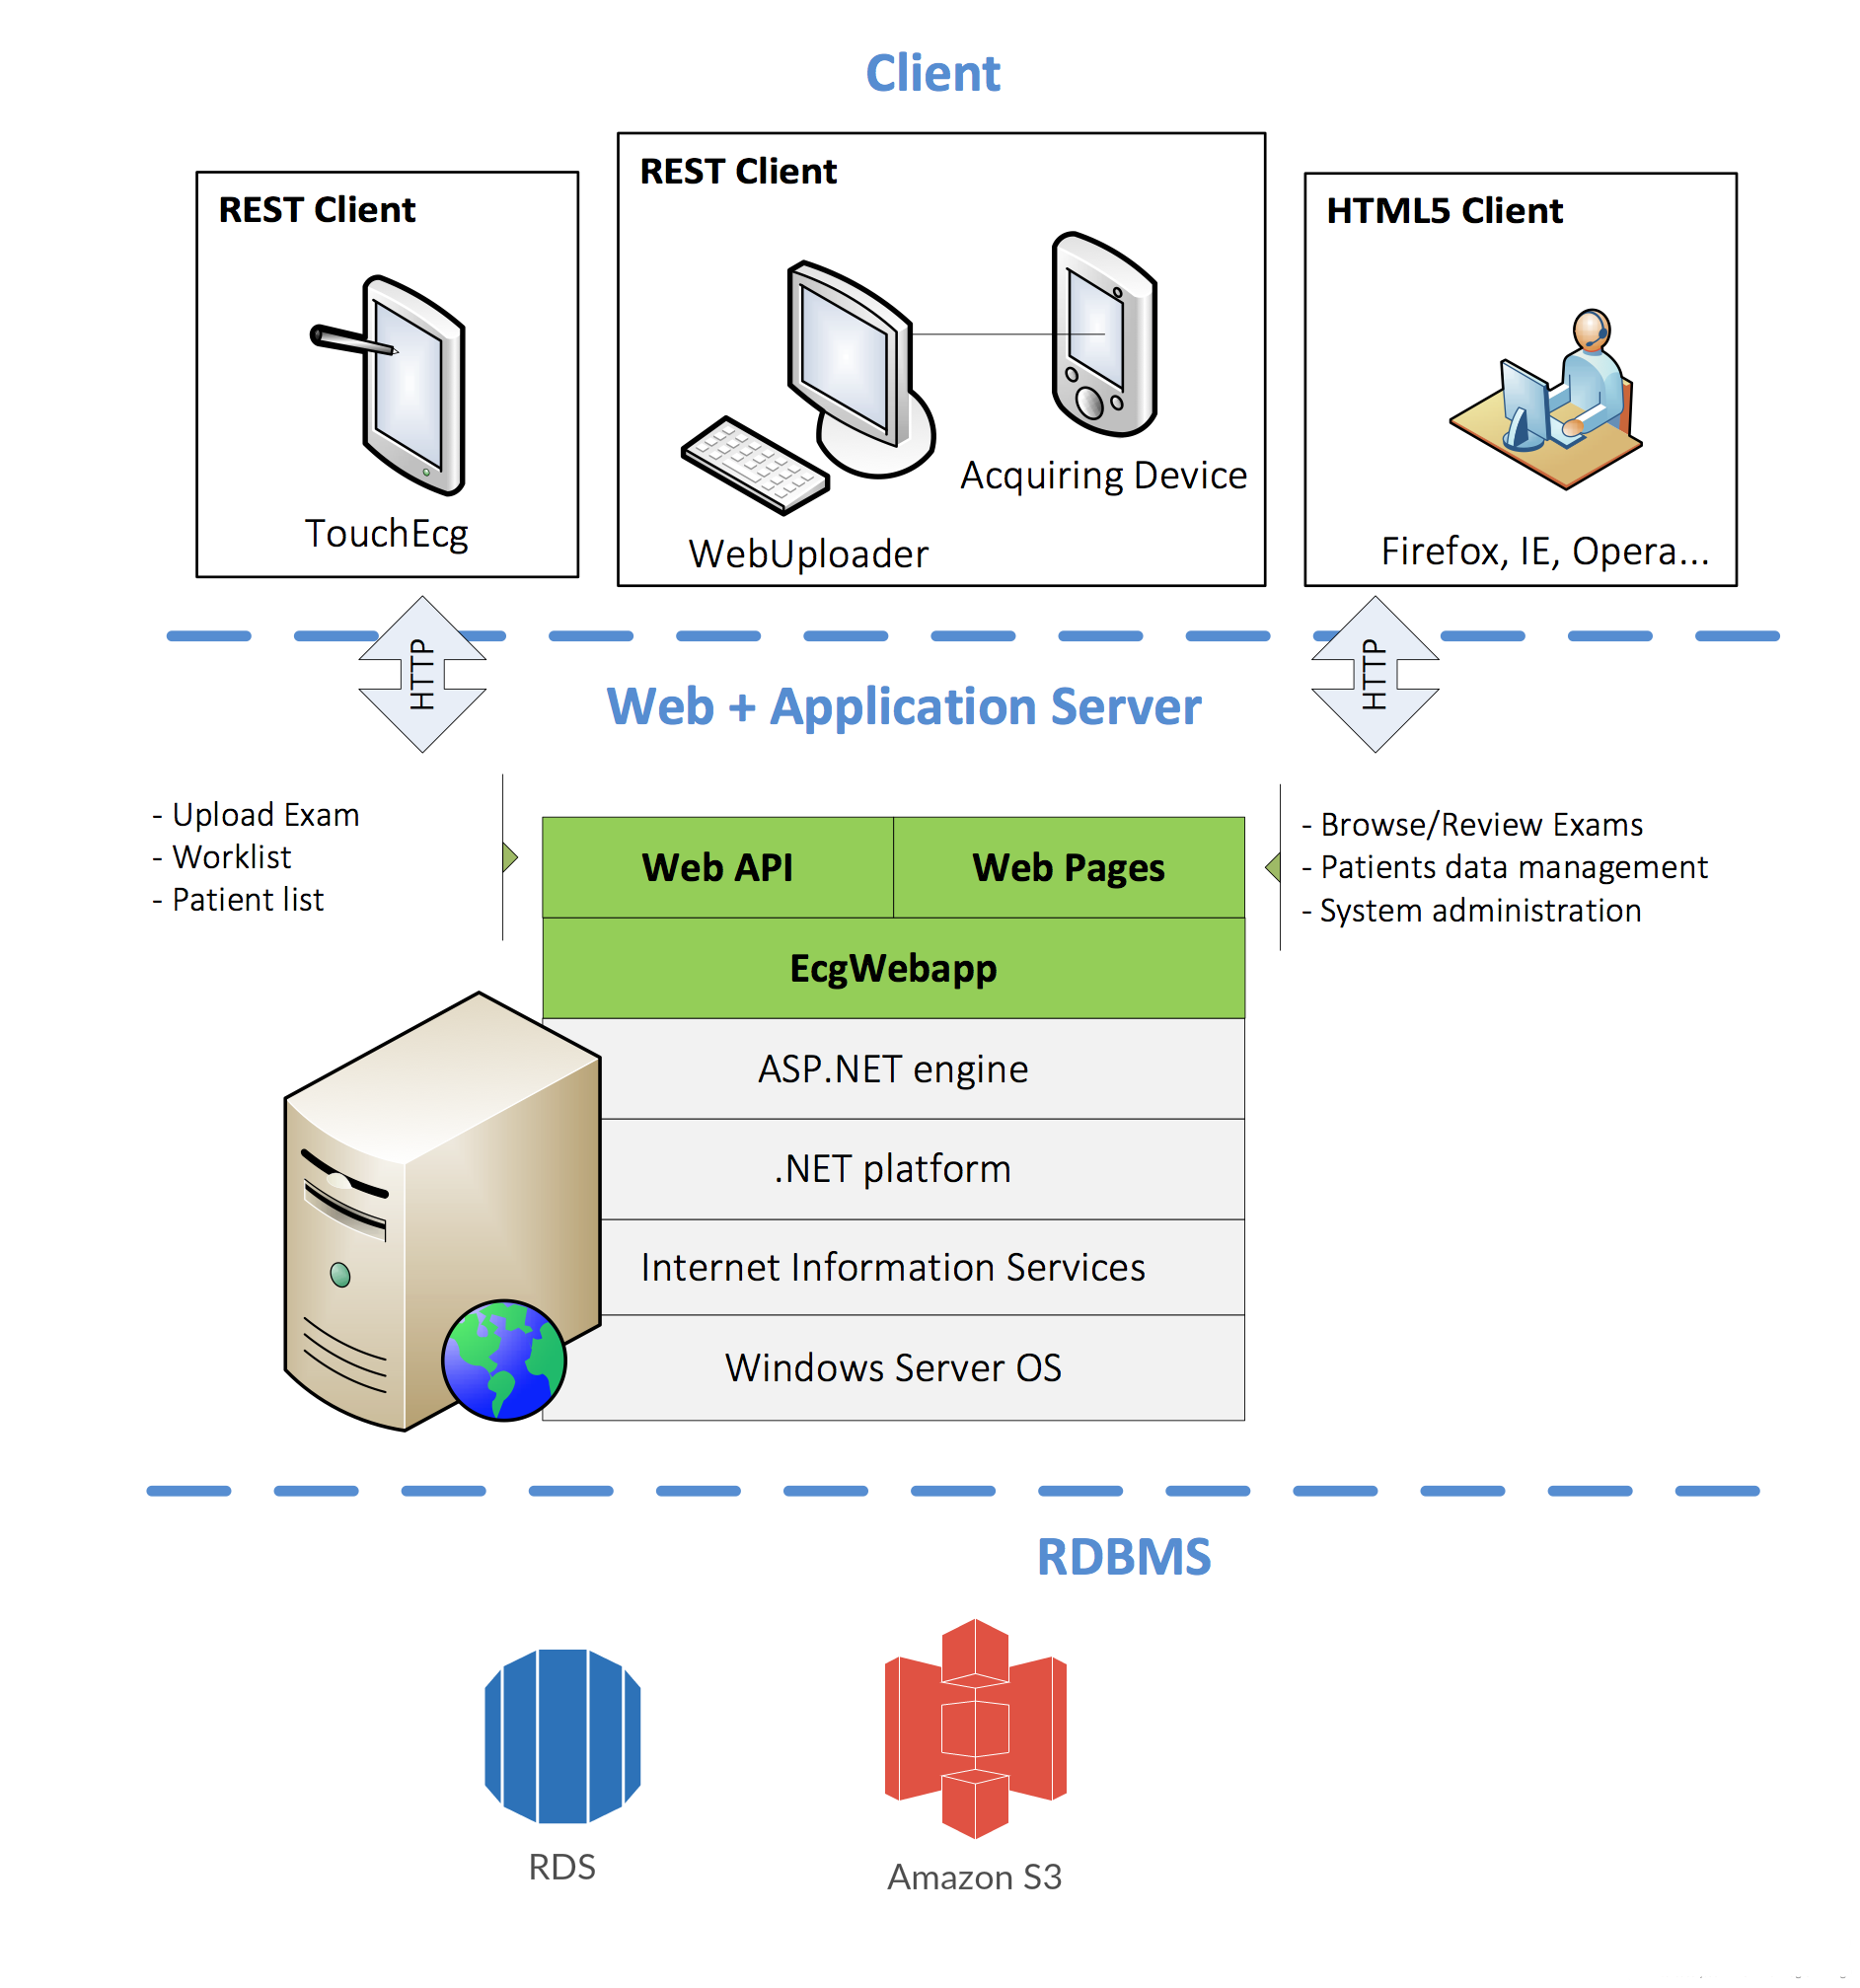
\includegraphics[width=\textwidth,height=10cm,keepaspectratio]{img/tiers_diagram}
    \caption{3-tier architecture}
    \label{fig:tiers_diagram}
\end{figure}
The MVC \textit{(Model View Controller)} paradigm allows to isolate the domain specific logic from the input and presentation ones, making testing and development easier. \cite{mvc}\\
In this specific context the \textit{model} includes objects as exams and patients and their relations, which are mapped to MySql Database Entities by Entity Framework (EF), an open source object-relational-mapping tool (ORM) developed by Microsoft, in order to work without taking care of the underlying database tables and columns where data are actually stored. Indeed developers deal with an higher level of abstraction \cite{wikipedia_ef}.\\
The \textit{view} manages data presentation, serving html pages or json formatted data, as show in figure \ref{fig:app_resource_pattern}.\\
\begin{figure}[h]
    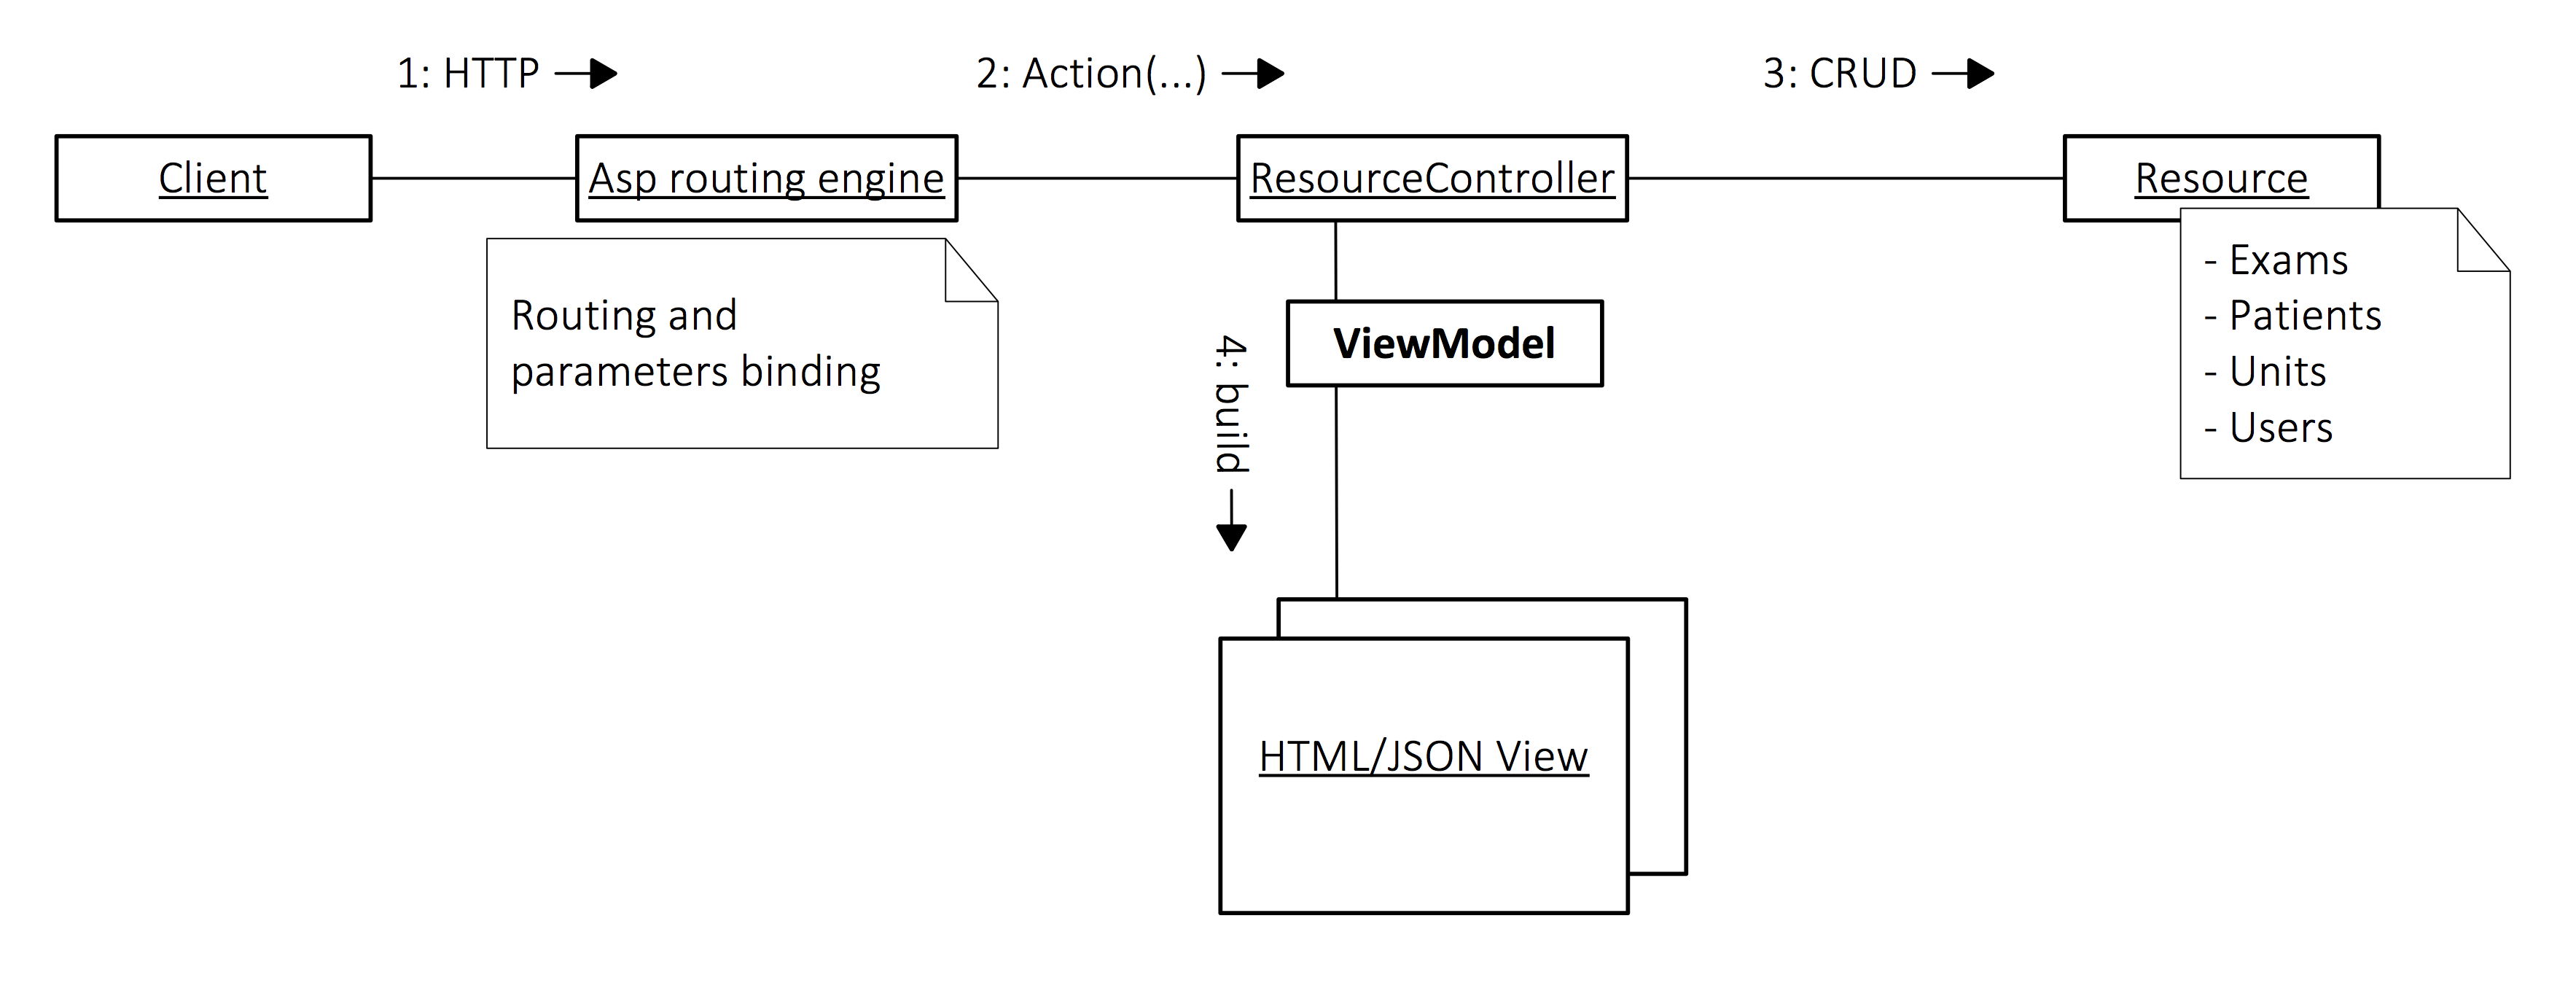
\includegraphics[width=\textwidth]{img/app_resource_pattern}
    \caption{Each application resource has been implemented following this pattern}
    \label{fig:app_resource_pattern}
\end{figure}
WebServices included in EcgWebApp are based on the ASP .NET WebApi Framework, a REST interface triggers a specific action on a resource depending on the URL parameters and the HTTP verb used. Basic Authentication is used to provide access control to web resources.\\ \\
A specific module has been developed to prepare reviewed electrocardiograms for the 
\paragraph{Ecg Web Receiver}
\label{paragraph:ecgwebreceiver}
Similarly to EcgWebApp, (\ref{paragraph:ecgwebapp}) Ecg WebReceiver is an ASP .NET MVC application with a REST webservice module developed with WebApi framework.\\
To receive large files the client must firstly ask WebReceiver for an upload-session token id, then it starts sending chunks of data until the second last one, each time communicating the uploading session id, finally the client sends the very last chunks and commits uploading (for a diagram see fig.\ref{fig:holter_sequence_diagram}). Each requests made by client is authenticated server-side from a basic-authentication mechanism., the user is then identified and the exam loaded to the associated bucket on Amazon Simple Storage Service (S3).
The system admin is allowed to login and perform CRUD on users and buckets resources from a web based user interface (screenshot at fig. \ref{fig:webreceiver_admin_screenshot})

\clearpage

\subsection{Clients}
Here is presented a set of client applications which interact with the previously defined components, EcgWebApp (\ref{paragraph:ecgwebapp}) and Ecg WebReceiver (\ref{paragraph:ecgwebreceiver}) over the HTTP protocol.
\paragraph{Touch Ecg}
Touch Ecg is a Cardioline electrocardiograph 12-lead (more details for 12-lead at \ref{subsection:12leadecg}) application for tablet PC, it acquires raw electrocardiograms data from the compatible devices, which are eventually analysed later by the \textit{"Glasgow"} \cite{glasgow} interpretation algorithm.\\
After a configuration phase, where the user is asked to provide the endpoint which the waveforms should be uploaded to, it is possible to transfer ECG-SCP (informations about SCP-ECG file format at \ref{subsection:ecgdigitaliation}) files via a REST WebService (\ref{paragraph:REST}).
\paragraph{Web Uploader}
It is a stand-alone client application developed specifically to save, from Cardioline devices, long time registrations, as Holters are, and upload them. Because the length of such documents an upload protocol has been built to ensure all data reach the WebReceiver endpoint, illustrated in fig. \ref{fig:holter_sequence_diagram}.
\begin{figure}[h]
    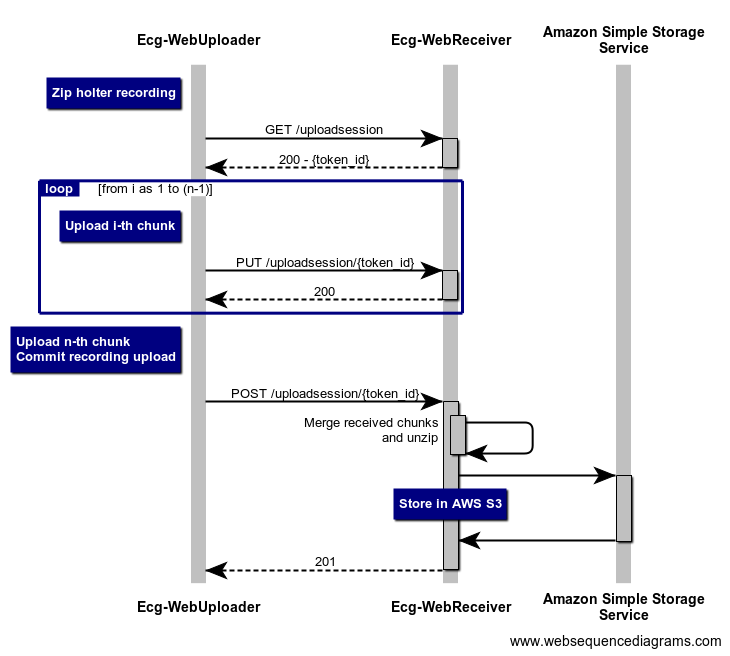
\includegraphics[width=\textwidth]{img/holter_sequence_diagram}
    \caption{Sequence diagram for Holter exams uploading}
    \label{fig:holter_sequence_diagram}
\end{figure}
\paragraph{Browser}
Any browser application can access web pages provided by EcgWebApp (\ref{paragraph:ecgwebapp}), in this way each tenant user is able to login via his/her own computer without installing any additional software, from anywhere.
Here the Ecg-Workflow described in \ref{section:ecgworkflow} is implemented and available to different users.\\
\paragraph{Cube Holter}
An ad hoc software for in-depth holter exam review, given a folder it looks up for the available exams inside.
Because Cardioline tools used to be hosted on a LAN it was easier to deliver directly a long-time heart activity recording to the machine which would be used for the analysis, given the architectural change carried out, legacy software as CubeHolter have been provided with a module which creates a virtual storage device synchronized with the related Amazon Simple Storage S3 bucket where exams are exported by WebReceiver (\ref{paragraph:ecgwebreceiver}), hence the tool configured to look for exams in such virtual device, the result is a user transparent synchronization mechanism between local machines and cloud even for large files.

\section{Screenshots}

\begin{figure}[h]
    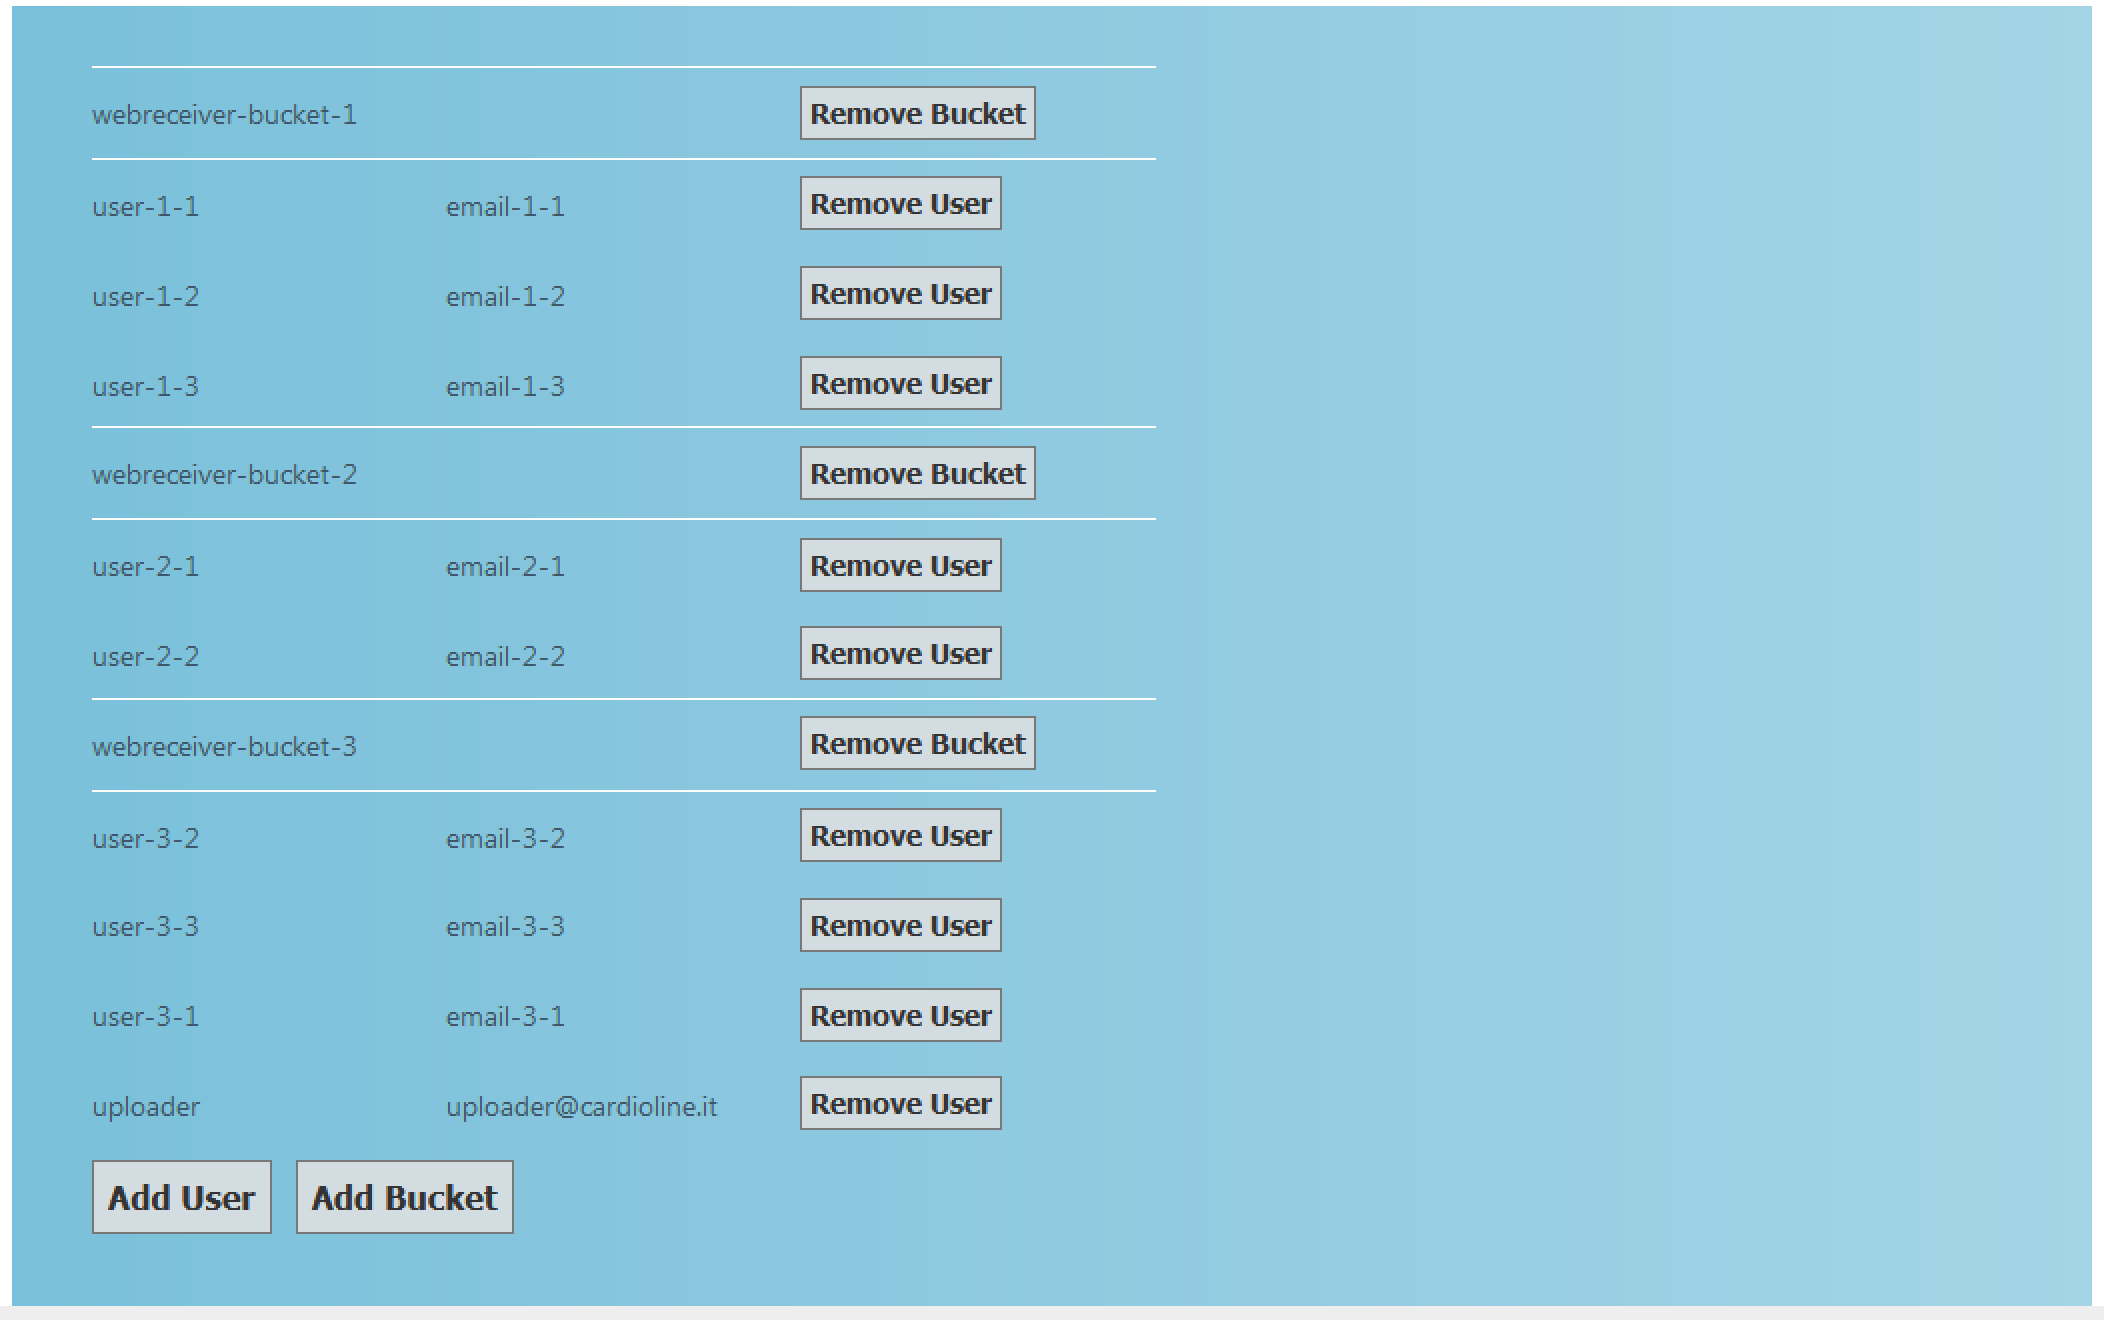
\includegraphics[width=\textwidth]{img/webreceiver_admin_screenshot}
    \caption{Admin user interface for buckets and users management}
    \label{fig:webreceiver_admin_screenshot}
\end{figure}

\begin{figure}[h]
    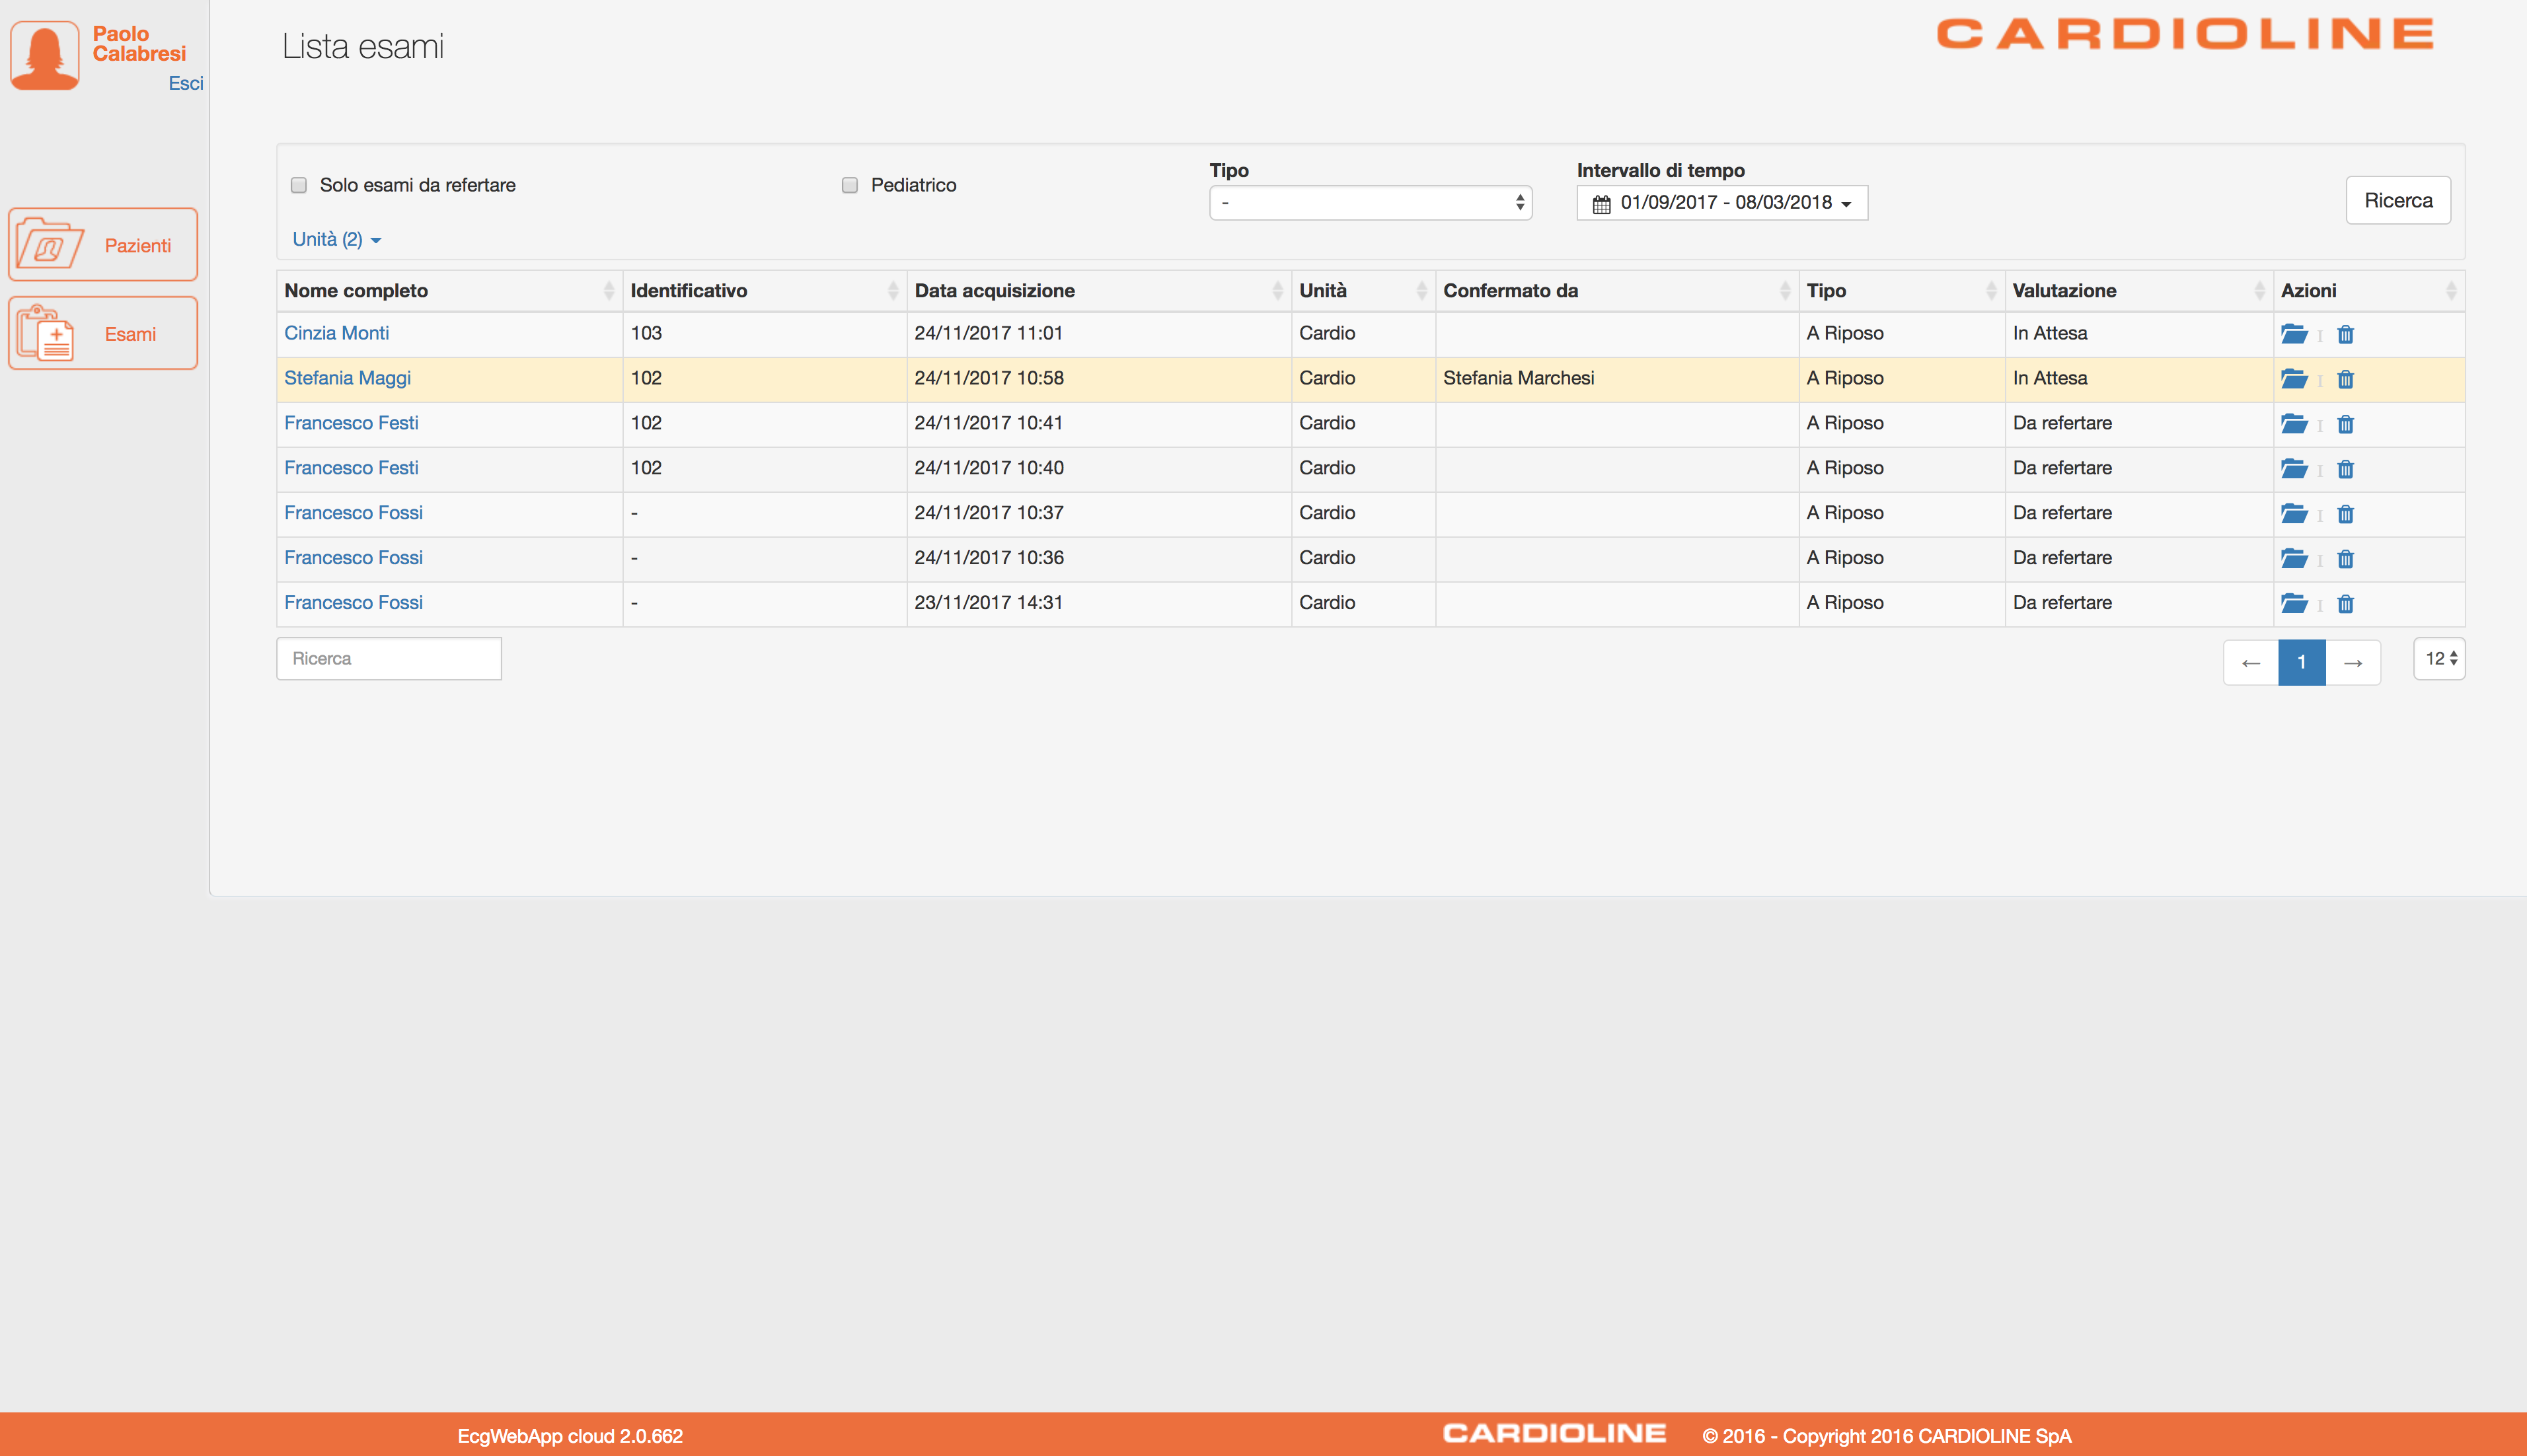
\includegraphics[width=\textwidth]{img/todo_anamnesi}
    \caption{User interface showing anamnesis needed}
    \label{fig:todo_anamnesi}
\end{figure}

\begin{figure}[h]
    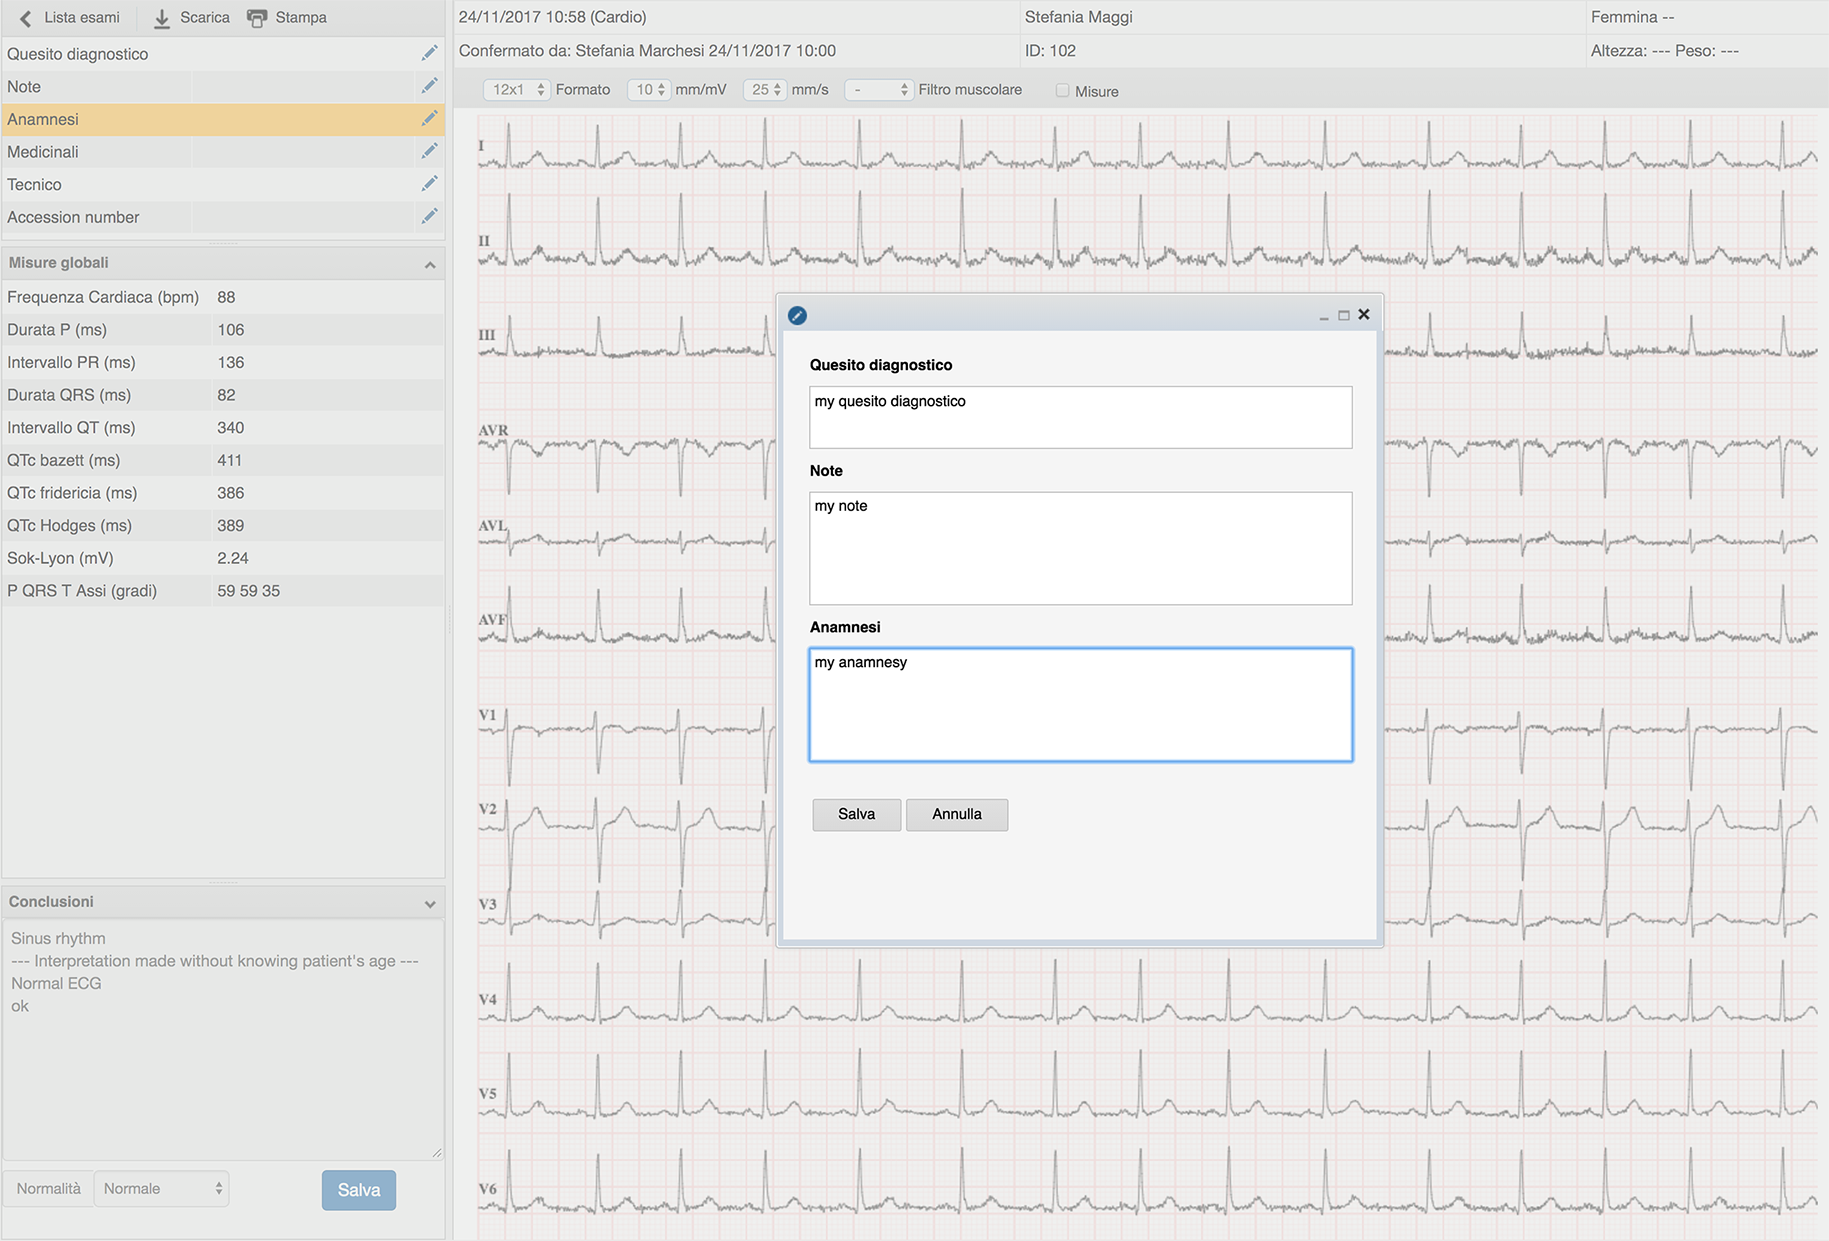
\includegraphics[width=\textwidth]{img/aggiunta_anamnesi}
    \caption{User interface showing anamnesis provisioning}
    \label{fig:aggiunta_anamnesi}
\end{figure}

\begin{figure}[h]
    \includegraphics[width=\textwidth]{img/refertazione_esame}
    \caption{Conclusion provisioning user interface}
    \label{fig:refertazione_esame}
\end{figure}




      \chapter{Conclusions}
\section{Produced Improvement}
Even in a complex field as e-health is because sensible data, different country legislations and lots of specific standards each one with pro and cons coming from past years of un-coordinated developement. The current technological landscape is slowly converging among formats, interfaces and protocols, thanks to the succesful spread of distributed systems and web services.\\
Starting from proprietary softwares each one partecipating to an e-health system, as the Cardioline one described in \ref{chapter:cardioline_specific_ecosystem}, bounded to each customer company or organization and ending up with a cloud based system (see chapter \ref{chapter:implemented_solution}) which strongly uses international standard to store data and communicate with external services and devices breaking physical barriers in time and space, can be considered a consistent improvement.\\
Especially for companies which work with digital healthcare data, is important to underline the real possibility to provide each one softwares, even the legacy ones, with ad hoc modules to map their data into modern standards and EHR repository compliant formats, without radically changing their currrent workflow.
The adoption of standard communication architecture is at the same way very useful to enable interactions with the widest possible set of external devices, decreasing the time needed to complete specific tasks.\\ \\
The developement of this prototype is valuable not only for Cardioline as a company but also as an experiment to break the current digital healthcare barriers.\\
Concluding, the economic and time effort required for this kind of evolution, has to be as lowest as possible, in particular dealing with e-health which is already strongly limited by countries and organizations burocracy. Hence the usage of cloud computing environment because their optimized resource consuption and cost brings a great technological and business advantage.

\section{Future Develompent}
Once countries EHR will be opened to third-party stakeholders, the prototype developed in Cardioline will be immediately able to send its own produced documents through an appropriate communication channel.
Cardioline is still focused on improving the developed prototype, in details, to respect the future European Law about privacy and sensible data it will be necessary to implement a strong-authentication mechanism and enable cardiologists to sign digitally.\\
Furthermore a deep testing has to be done in order to analyse the system behaviour in case of huge treffic and resources demand.
      
      
      
      
      
    \endgroup


    % bibliografia in formato bibtex
    %
    % aggiunta del capitolo nell'indice
    \addcontentsline{toc}{chapter}{Bibliografia}
    % stile con ordinamento alfabetico in funzione degli autori
    
    \bibliography{biblio}
    \bibliographystyle{plain}
%%%%%%%%%%%%%%%%%%%%%%%%%%%%%%%%%%%%%%%%%%%%%%%%%%%%%%%%%%%%%%%%%%%%%%%%%%
%%%%%%%%%%%%%%%%%%%%%%%%%%%%%%%%%%%%%%%%%%%%%%%%%%%%%%%%%%%%%%%%%%%%%%%%%%
%% Nota
%%%%%%%%%%%%%%%%%%%%%%%%%%%%%%%%%%%%%%%%%%%%%%%%%%%%%%%%%%%%%%%%%%%%%%%%%%
%% Nella bibliografia devono essere riportati tutte le fonti consultate 
%% per lo svolgimento della tesi. La bibliografia deve essere redatta 
%% in ordine alfabetico sul cognome del primo autore. 
%% 
%% La forma della citazione bibliografica va inserita secondo la fonte utilizzata:
%% 
%% LIBRI
%% Cognome e iniziale del nome autore/autori, la data di edizione, titolo, casa editrice, eventuale numero dell’edizione. 
%% 
%% ARTICOLI DI RIVISTA
%% Cognome e iniziale del nome autore/autori, titolo articolo, titolo rivista, volume, numero, numero di pagine.
%% 
%% ARTICOLI DI CONFERENZA
%% Cognome e iniziale del nome autore/autori (anno), titolo articolo, titolo conferenza, luogo della conferenza (città e paese), date della conferenza, numero di pagine. 
%% 
%% SITOGRAFIA
%% La sitografia contiene un elenco di indirizzi Web consultati e disposti in ordine alfabetico. 
%% E’ necessario:
%%   Copiare la URL (l’indirizzo web) specifica della pagina consultata
%%   Se disponibile, indicare il cognome e nome dell’autore, il titolo ed eventuale sottotitolo del testo
%%   Se disponibile, inserire la data di ultima consultazione della risorsa (gg/mm/aaaa).    
%%%%%%%%%%%%%%%%%%%%%%%%%%%%%%%%%%%%%%%%%%%%%%%%%%%%%%%%%%%%%%%%%%%%%%%%%%
%%%%%%%%%%%%%%%%%%%%%%%%%%%%%%%%%%%%%%%%%%%%%%%%%%%%%%%%%%%%%%%%%%%%%%%%%%
    

    \titleformat{\chapter}
        {\normalfont\Huge\bfseries}{Allegato \thechapter}{1em}{}
    % sezione Allegati - opzionale
    \appendix
    \chapter{Titolo primo allegato}

Lorem ipsum dolor sit amet, consectetur adipiscing elit. Donec sed nunc orci. Aliquam nec nisl vitae sapien pulvinar dictum quis non urna. Suspendisse at dui a erat aliquam vestibulum. Quisque ultrices pellentesque pellentesque. Pellentesque egestas quam sed blandit tempus. Sed congue nec risus posuere euismod. Maecenas ut lacus id mauris sagittis egestas a eu dui. Class aptent taciti sociosqu ad litora torquent per conubia nostra, per inceptos himenaeos. Pellentesque at ultrices tellus. Ut eu purus eget sem iaculis ultricies sed non lorem. Curabitur gravida dui eget ex vestibulum venenatis. Phasellus gravida tellus velit, non eleifend justo lobortis eget. 

\section{Titolo}
Lorem ipsum dolor sit amet, consectetur adipiscing elit. Donec sed nunc orci. Aliquam nec nisl vitae sapien pulvinar dictum quis non urna. Suspendisse at dui a erat aliquam vestibulum. Quisque ultrices pellentesque pellentesque. Pellentesque egestas quam sed blandit tempus. Sed congue nec risus posuere euismod. Maecenas ut lacus id mauris sagittis egestas a eu dui. Class aptent taciti sociosqu ad litora torquent per conubia nostra, per inceptos himenaeos. Pellentesque at ultrices tellus. Ut eu purus eget sem iaculis ultricies sed non lorem. Curabitur gravida dui eget ex vestibulum venenatis. Phasellus gravida tellus velit, non eleifend justo lobortis eget. 

\subsection{Sottotitolo}
Lorem ipsum dolor sit amet, consectetur adipiscing elit. Donec sed nunc orci. Aliquam nec nisl vitae sapien pulvinar dictum quis non urna. Suspendisse at dui a erat aliquam vestibulum. Quisque ultrices pellentesque pellentesque. Pellentesque egestas quam sed blandit tempus. Sed congue nec risus posuere euismod. Maecenas ut lacus id mauris sagittis egestas a eu dui. Class aptent taciti sociosqu ad litora torquent per conubia nostra, per inceptos himenaeos. Pellentesque at ultrices tellus. Ut eu purus eget sem iaculis ultricies sed non lorem. Curabitur gravida dui eget ex vestibulum venenatis. Phasellus gravida tellus velit, non eleifend justo lobortis eget. 


\chapter{Titolo secondo allegato}

Lorem ipsum dolor sit amet, consectetur adipiscing elit. Donec sed nunc orci. Aliquam nec nisl vitae sapien pulvinar dictum quis non urna. Suspendisse at dui a erat aliquam vestibulum. Quisque ultrices pellentesque pellentesque. Pellentesque egestas quam sed blandit tempus. Sed congue nec risus posuere euismod. Maecenas ut lacus id mauris sagittis egestas a eu dui. Class aptent taciti sociosqu ad litora torquent per conubia nostra, per inceptos himenaeos. Pellentesque at ultrices tellus. Ut eu purus eget sem iaculis ultricies sed non lorem. Curabitur gravida dui eget ex vestibulum venenatis. Phasellus gravida tellus velit, non eleifend justo lobortis eget. 

\section{Titolo}
Lorem ipsum dolor sit amet, consectetur adipiscing elit. Donec sed nunc orci. Aliquam nec nisl vitae sapien pulvinar dictum quis non urna. Suspendisse at dui a erat aliquam vestibulum. Quisque ultrices pellentesque pellentesque. Pellentesque egestas quam sed blandit tempus. Sed congue nec risus posuere euismod. Maecenas ut lacus id mauris sagittis egestas a eu dui. Class aptent taciti sociosqu ad litora torquent per conubia nostra, per inceptos himenaeos. Pellentesque at ultrices tellus. Ut eu purus eget sem iaculis ultricies sed non lorem. Curabitur gravida dui eget ex vestibulum venenatis. Phasellus gravida tellus velit, non eleifend justo lobortis eget. 

\subsection{Sottotitolo}
Lorem ipsum dolor sit amet, consectetur adipiscing elit. Donec sed nunc orci. Aliquam nec nisl vitae sapien pulvinar dictum quis non urna. Suspendisse at dui a erat aliquam vestibulum. Quisque ultrices pellentesque pellentesque. Pellentesque egestas quam sed blandit tempus. Sed congue nec risus posuere euismod. Maecenas ut lacus id mauris sagittis egestas a eu dui. Class aptent taciti sociosqu ad litora torquent per conubia nostra, per inceptos himenaeos. Pellentesque at ultrices tellus. Ut eu purus eget sem iaculis ultricies sed non lorem. Curabitur gravida dui eget ex vestibulum venenatis. Phasellus gravida tellus velit, non eleifend justo lobortis eget. 




\end{document}